\section{Requirements}
\label{sec:requirements}

Sampling the Gaussian process prediction forumula \autoref{eq:gp-pred} directly
in sufficient density to draw the slices is expensive because each evaluation
requires computing the dot product of two size $N$ vectors.  Instead, I render
the prediction formula in order to exploit the inherent parallelism provided by
the GPU. Before describing the algorithm itself, we first need to consider what
the multi-dimensional ``scene'' we are trying to render looks like.  The
fundamental data type we are given are sample points of the simulation.  This
section describes how these sample points are transformed into higher-order
geometric primitives and then what happens when slicing them in order to be
drawn on screen.

\subsection{Scene geometry}
\label{sec:scene_geometry}

Here I will describe the spatial interpretation of the Gaussian process
model so that one can build an intuition for the geometric portion of the 
prediction formula.  This spatial interpretation is very close to the 
form used for the splatting algorithm.

The spatial interpretation of the Gaussian process model using squared 
exponential correlation is a set of 
multi-dimensional ellipsoids, one for each sample point. 
One may be tempted to think this is due to uncertainty at the sample points
but this is not the case here as the outputs of a computer simulation are
considered exact. The ellipsoids are due to giving the correlation functions
compact support.
In order to see
why this is the case we first begin by looking at the formula for the 
``best linear unbiased prediction,''
at an arbitrary location
in the parameter space, $x'$, which is,

\begin{align}
  \hat{y}(x') &= \mu + \vec{r}(x') R^{-1} (\vec{Y} - \mu)' \text{,}
  \label{eq:gp-pred}
\end{align}
here $\vec{r}$ is a vector of functions, one per sample point
and each element of $r$, $r_i$, is the correlation 
between
sample point $x_i$ and $x'$.  
$\vec{Y}$ is a vector of the sampled outputs.
$\mu$ is the estimated process mean.
$R$ is 
the $N \times N$ correlation matrix 
between the sample points using the same correlation function.
We also note that neither $R^{-1}$ nor $(Y - \mu)$
depend on $x'$ so let the vector, 
$\vec{\Upsilon} = R^{-1} (\vec{Y} - \mu)'$.  
Then, we can write \autoref{eq:gp-pred} in a linear form,

\begin{align*}
  \hat{y}(x') &= \mu + r(x') \vec{\Upsilon} \\
              &= \mu + \sum_{i=1}^N r_i(x') \Upsilon_i \text{.}
\end{align*}
The value $\Upsilon_i$ is $f'(x_i)$ and $\hat{y}$ is $\hat{f}$ from 
\autoref{eq:kernel_regression} which is normalized by $R^{-1}$ from 
\autoref{eq:gp-pred}.

A common choice for $r(\cdot)$ is the squared exponential correlation
function
which has infinite support and is strictly 
positive meaning that it is defined everywhere in the domain and always 
returns some positive value however small. 
There is a different falloff
parameter for each dimension.
For visualization purposes these small values don't contribute a
perceivable effect.
Therefore, I set a lower bound on the correlation value which we denote,
$\epsilon = 1 \times 10^{-9}$, essentially giving the correlation function
compact support. This can also be done using specific compactly supported 
correlation functions as in
Kaufman et al.~\cite{Kaufman:2011}. 
The squared exponential correlation function is radial meaning the
correlation amount between points decreases as the distance increases.
This $\epsilon$ value essentially creates a $d$-dimensional ellipsoid region
around each sample point with principal axis lengths related to the 
correlation falloff parameter. The sample point will only influence 
predictions within this region.

\subsection{HyperSlice effect on scene geometry}
\label{sec:hypersliceeffectonscenegeometry}

The last step is using some method to examine this multi-dimensional
scene on a computer screen. My
chosen display method is the
HyperSlice~\cite{Wijk:1993} technique to which will draw $2$-dimensional
slices through these multi-dimensional ellipsoids on screen.  
HyperSlice relies on the user selecting a \textit{viewpoint} which 
determines the location in the multi-dimensional parameter space where to
position of the slices.
In \autoref{fig:hyperslice_geometry} I show the representation for the
HyperSlice technique in both 2 and 3 dimensions.  In 2D the slicing plane (what
one sees) is a line.  In 3D it is a 2D plane slicing through the space.  In 
higher dimensions it is also a 2D slicing plane.

\begin{figure}[htb]
  \centering
  \begin{subfigure}{0.45\linewidth}
    \centering
    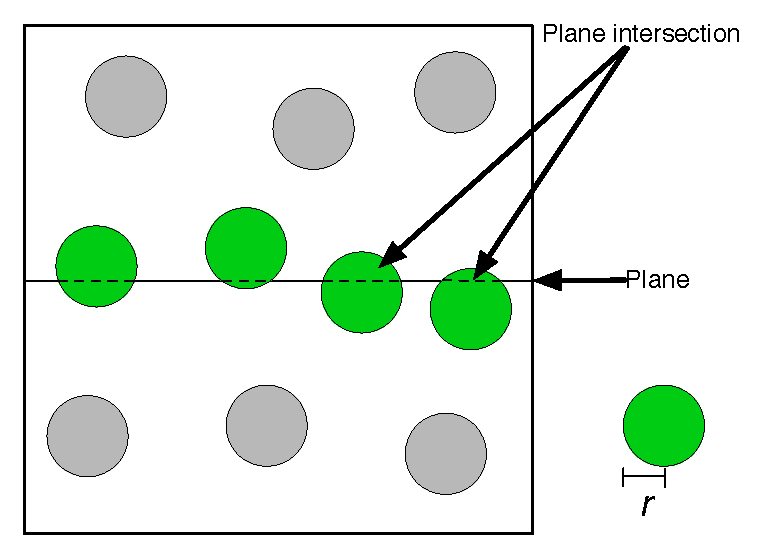
\includegraphics[width=\linewidth]{gp_diagram_2d}
    \caption{2D view}
    \label{fig:hs_2d}
  \end{subfigure}%
  \begin{subfigure}{0.45\linewidth}
    \centering
    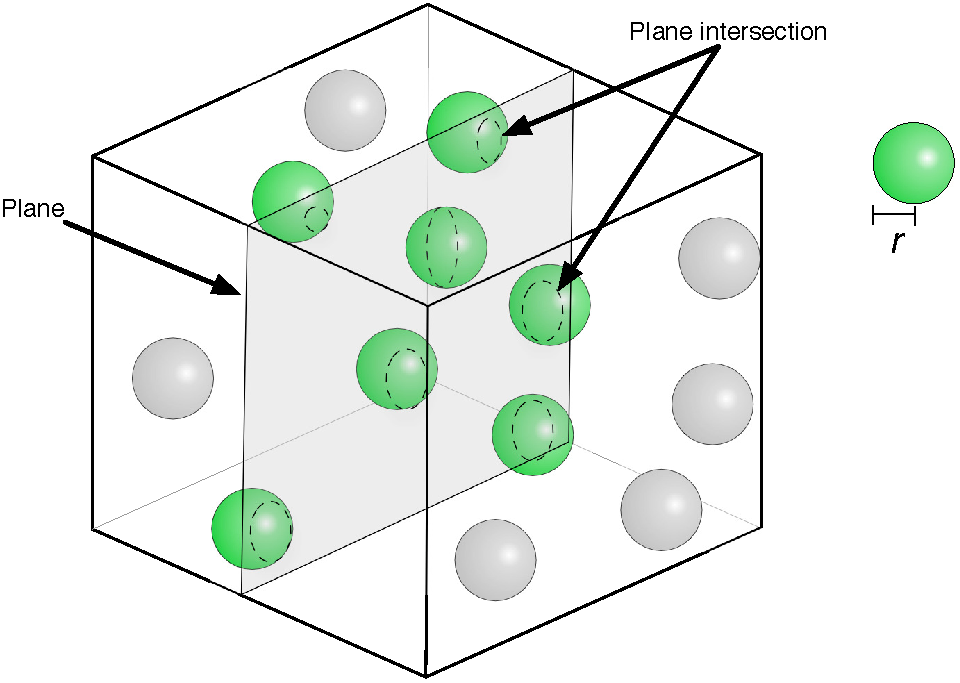
\includegraphics[width=\linewidth]{gp_diagram_3d}
    \caption{3D view}
    \label{fig:hs_3d}
  \end{subfigure}
  \caption[Example of 2D slices of 2D and 3D spheres]{
    Diagrams showing how the HyperSlice~\cite{Wijk:1993} method ``slices'' 
    through the 
    kernels of the Gaussian process model in both 2D (a) and 3D (b).  The 
    slicing plane is denoted as ``Plane'' in the figure.  This is the 
    plane the user views.  Only the points, denoted in green, fall within a 
    distance $r$ of the slicing
    plane will influence the rendered image.  All other points can be filtered
    out as they do not affect the image.  We then compute the influence of 
    the unfiltered (green) points on the slicing plane.
  }
  \label{fig:hyperslice_geometry}
\end{figure}


Only the points within range $r$ of the slicing plane have an effect on the
final image on the slice.
The conceptual algorithm works by first filtering out all points
that do not fall within range, $r$, of the slicing plane.  Then, for all points
within this range, I determine where the drawing plane intersects the
ellipsoid which determines its impact on the drawing plane.

\subsection{Algorithm}

The GPU has vertex and fragment processing stages.  This is analogous
to the filtering and rendering stages of our rendering algorithm.
I present the full schematic of the rendering algorithm in \autoref{algo:full}.

The distance to the slice is a $d-2$ dimensional distance since the remaining
$2$ dimensions are projected on to the slice directly.
I compute the projection of the point onto the current 2D 
slice in~\autoref{algo:full} (\autoref{al:line:slicedist}).
I then compute the distance of the sample point to the slice in 
\autoref{al:line:disteq}.
Because I am only interested in the distance to the slice itself, and not
a particular point on that slice, I don't include the two dimensions
of the slice in the distance computation.  
If this distance is smaller
than the size of the reconstruction kernel, I render a
2D slice through this reconstruction kernel. 
A speed-up for drawing exponential functions often used
in GPU-based splatting algorithms is to use a template exponential distribution
drawn onto a quad~\cite{Mueller:1998}.
However, since these splat-like slices have different distances from each subplot they affect
the subplot by different amounts depending on the distance.  Therefore, I
need to scale the intensity
value of the texture by its distance to the 
slice (\autoref{al:line:splatscale}).

\begin{algorithm}
  \caption{Rendering multi-dimensional data using HyperSlice and Gaussian process regression}
  \label{algo:full}
  \begin{algorithmic}
  \Require viewpoint $\vec{v}$, maximum distance $r$
  \Ensure ${d \choose 2}$ slices through an $N$-point, $d$-dimensional data set
  \ForAll {${d \choose 2}$ subplots $S_i$} \Comment{filtering}
    \ForAll {$N$ points $p$ in the vertex buffer}
      \State $p_{2D} \gets$ the 2D projection of $p$ onto the slice $S_i$\label{al:line:slicedist}\;
      \State $\mathrm{dist} \gets$ the distance of $p$ to the slice $S_i$\label{al:line:disteq}\;
      \If {$\mathrm{dist} < r$} \Comment{rendering} \label{al:line:filterif}
        \State $\mathrm{tex} \gets$ the Gaussian splat scaled by $\mathrm{dist}$\label{al:line:splatscale}\;
        \State $\hat{p}_{2D} \gets$ transform $p_{2D}$ into screen coordinates\label{al:line:screenpoint}\;
        \State $w \gets$ compute the splat width ($\sqrt{r^2-\mathrm{dist}^2}$)\label{al:line:splatsize}\;
        \State send 2D quads $(\hat{p}_{2D}(x) \pm w, \hat{p}_{2D}(y) \pm w)$ to the 
          fragment shader to be shaded with $\mathrm{tex}$\;
      \EndIf
    \EndFor
  \EndFor
  \end{algorithmic}
\end{algorithm}

In my vertex shader implementation I filter the points as well as compute
the sliced splat size.  This splat size is used to generate a quad that I
send to the fragment shader.  I use the fragment shader to compute the 
final pixel color values within the slice.
For practical visualizations this final pixel color value should be passed
through a colormap.  Therefore, in such practical applications, I recommend
rendering the pixel values to a floating point texture. Then this floating
point texture can be rendered to the screen with a colormap shader program
to convert the floating point values to color values.

One of the main bottlenecks in the rendering pipeline is transferring
vertex data from CPU memory to GPU memory.  This is due to the slower
speed of the bus compared to the GPU. I do not want the GPU waiting
for pixel data.  The best way to address this, as specified by Xue and
Crawfis~\cite{Xue:2003}, is to store vertex data in display lists on the
GPU.  Then, before calling a draw command, I only need to update the 
small amount of viewpoint information to
render the group of slices to the GPU. Hence, I store all $N$ $d$-dimensional
data points on the GPU. Memory of current GPUs is large enough that we can easily 
store millions of points in a number of dimensions directly on the card.

